\textbf{ButtonStyle.xaml}

Da \gls{KA} \gls{GUI} indeholder mange knapper, er der lavet en styling XAML fil for knapper, for at give \gls{KA} et mere karakteristisk udseende. Denne styling er også med til at dele de 3 segmenter i GUI'en mere op, og gøre det nemmere at benytte \gls{KA} intuitivt. \\
Styling filen består af RadialGradientBrushs, som giver knapperne et mere fysisk udseende. Styling filen er også tiltænkt at skulle give knapperne afrundede kanter.

\begin{figure}[H]
	\centering
	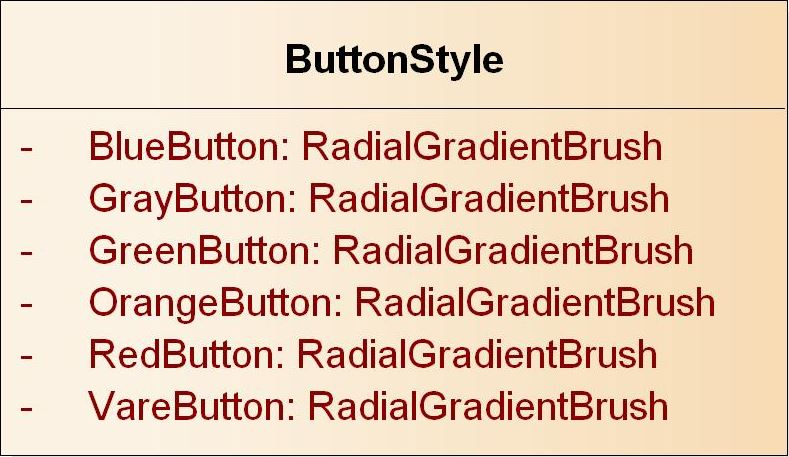
\includegraphics[width=60mm]{Systemdesign/Frontend/GUI/Pics/xaml}
	\caption{ButtonStyle.xaml}
	\label{fig:ButtonStyleXaml}
\end{figure}
